\section{Results}
In total 498 test cases were executed, totalling 24,900 packet transmissions. Of this total 19,545 were successfully received (78.5\%). The distribution of receive conditions for these individual points is indicated by Figure \ref{fig:density_plot}. Note that the raw \ac{rssi} values returned by the Radiohead library, and therefore the datalogger, are in fact packet strength for the SX1276 module; therefore a post-processing step has been applied to get separate packet strength and \ac{rssi} values valid for the RFM95W module. When discussing results, often received packets are considered alongside all other packets from the corresponding \ac{td}; this allows for metrics such as packet receive percentage (\ac{prp}) and average \ac{snr} to be used. Note that the logarithmic mean and standard deviation are used for decibel values.

\begin{figure}[H]
    \centering
   	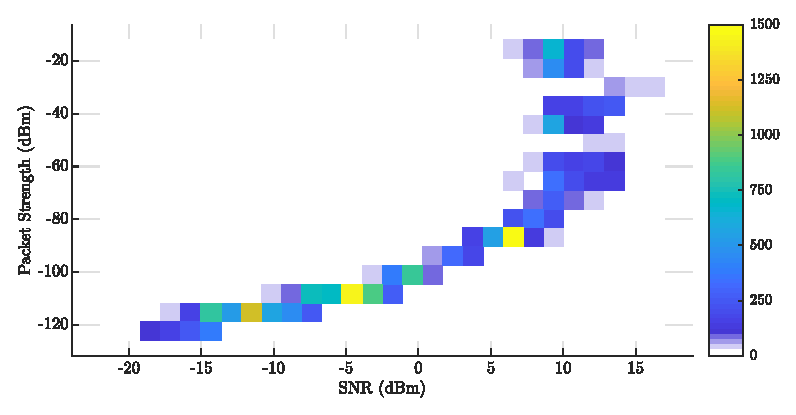
\includegraphics{Figures/density_plot}
    \caption[Test data distribution plot]{
    Density plot of received packet transmissions modelled as a bi-variate histogram with colour indicating received packet count. \\$Total\enskip Points = 19,545$
    }
    \label{fig:density_plot}
\end{figure}

\section{Discussion}
Results are considered in two domains: the demodulation performance of the radio, and the environment effects. This is done because, even though actual receive performance varies with factors such as distance and attenuation, these can be abstracted into changes of the underlying \ac{snr} and \ac{ps} figures seen by the receiver. As there are no other transmission sources in this testing, theoretically, if these figures are within the required bounds for demodulation success, receives are successful.

\subsection{Demodulation Performance}
When $\ac{snr} \leq 0$ the \ac{rssi} value indicates the amount of noise seen by the receiver in the presence of no packet. When operating at 868MHz, the noise that the receiver should see is approximately the thermal noise floor ($-174+10log_{10}(BW)$), plus the receiver noise figure; \ac{lora} implementations should have a noise figure of around 6dBm \cite{3YP:LORA_MOD_BASICS}. This indicates that for a 125kHz receive, the noise floor ($n_f$) should be -117dBm. The empirical noise floor calculated across all locations was -103dBm with a standard deviation of -109dBm; this is 14dBm ($24\times$) higher than expected. As the variance is low, this result indicates that the RFM95W hardware is of much poorer quality than expected, with a noise figure of 20dBm.

\begin{figure}[H]
    \centering
   	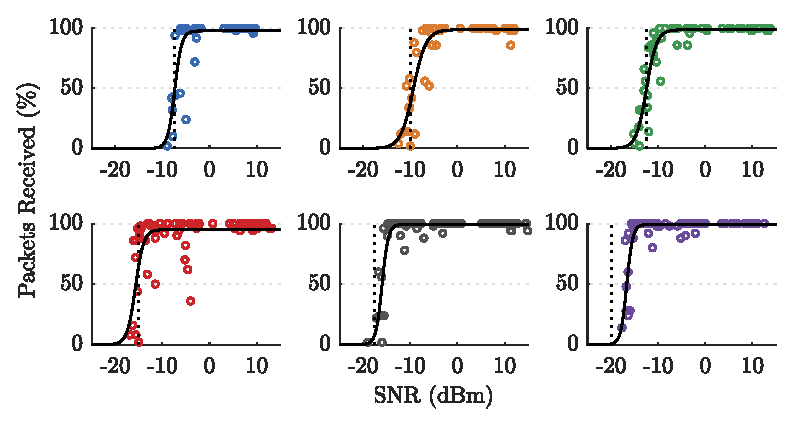
\includegraphics{Figures/sf_pp_separate_plot}
    \caption[Plots of \ac{snr} vs \ac{prp}]{
   \ac{td} mean \ac{snr} values plotted against their \ac{prp}s, separated by \ac{sf}s (Order = [[7, 8, 9], [10, 11, 12]]). For each \ac{sf} plot: the theoretical demodulation limit is indicated by the dotted line and the solid line corresponds to the best-fit sigmoid function; these are repeated in Figure \ref{fig:sf_pp_fit}. Although the best-fit sigmoids give a good representation of the general data pattern, and provide empirical demodulation cut-offs, they do not capture the high-variance receive behaviour when approaching the cut-off. This is reflected by the fact that only 62\%, 60\%, 66\%, 39\%, 77\% and 82\% of the respective training points fall inside the corresponding 95\% confidence interval.
   %Notably \ac{sf}10 has very high-variance; this is reflected in the 95\% maximum receive chance. 
    }
    \label{fig:sf_pp_separate}
\end{figure}
\vspace{-0.5cm}
Whether the radio receives a transmission is dictated by whether the received power exceeds the receiver sensitivity ($R_S$). For \ac{lora} modules, $R_S = n_f - \ac{sf}_{lim}$, where $SF_{lim}$ is the minimum SNR required for the current \ac{sf}. Theoretical limits are $-7.5, -10, -12.5, -15, -17.5, -20$ for $\ac{sf} = 7, 8, 9, 10, 11, 12$ respectively. This performance is explored in Figure \ref{fig:sf_pp_separate} and \ref{fig:sf_pp_fit}. In short, performance is close to theoretical for $\ac{sf} = 7, 8, 9, 10$ but $SF=11\enskip \& \enskip 12$ perform similarly to $SF=10$, just with higher reliably. For all configurations, receive success is highly variant when approaching the empirical sensitivity.

\begin{figure}[H]
    \centering
   	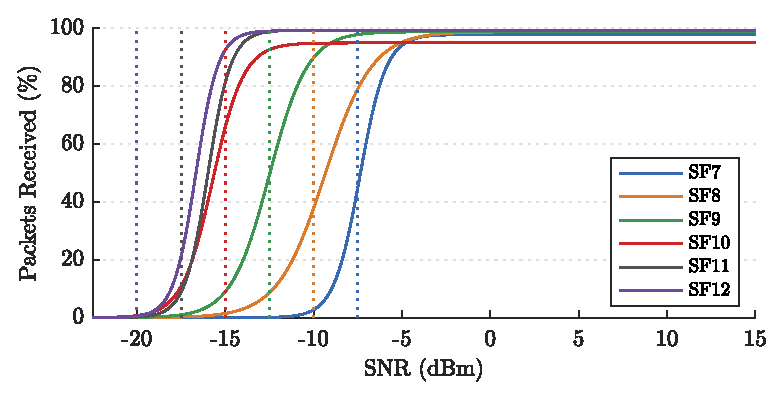
\includegraphics{Figures/sf_fit_plot}
    \caption[Sigmoid best-fits for \ac{snr} vs \ac{prp}]{
    Plot of sigmoid best-fits generated in Figure \ref{fig:sf_pp_separate}. The plot clearly demonstrates the positive effect increasing \ac{sf} has on demodulation performance of the receiver. For $\ac{sf}=7,8,9,10$ demodulation success starts dropping approximately 2.5dBm before the theoretical limit ($D_L$), with a 50\% \ac{prp} at $D_L$. This holds less so for \ac{sf}=11, for which drop-off starts around $D_L - 5dBm$, until $D_L$ where there is only a 10\% receive success. For \ac{sf}=12 drop-off starts around $D_L - 7.5dBm$, until $D_L$ where there is a 0\% receive success. Given the stable \ac{rssi} when $\ac{snr} < 0$, and that expected performance holds until a certain \ac{snr}, there is an indication that the sensitivity of the receiver is not as high as stated, possibly due to a cheap hardware implementation.
     }
    \label{fig:sf_pp_fit}
\end{figure}

Theoretically, higher \ac{cr}s will result in more data being recovered from a transmissions allowing for greater receive success. Comparative tests are plotted in Figure \ref{fig:cr_pp_plot}. As no strong visual conclusions can be made, a null hypothesis is proposed; $H_{0} : $ \textit{The mean \ac{prp} does not increase between receives using \ac{cr} 4/5 and \ac{cr} 4/8} (otherwise written as $4/5_{\ac{prp}} \geq 4/8_{\ac{prp}}$). The respective means are 71.8\% and 72.5\%. Using a left-tailed Wilcoxon signed rank test for non-normal distributions gives $p=41.2\%$. With a 5\% significance level,  $H_{0}$ cannot be rejected, indicating that \ac{cr} has no effect on \ac{prp}.  Given that the \ac{snr}s are not significantly different \textit{(hypothesis testing omitted)} this indicates that receive drop-off and high variance when approaching sensitivity limits is the limiting factor for demodulation. The lack of \ac{cr} effect is unsurprising given that \ac{fec}'s main performance should be seen in the presence of burst interference.

When the amount of data increases in a packet, its airtime will increase for the same configuration; this can lead to more channel noise being introduced (lower \ac{snr}) and receiver clock drift (lower demodulation performance). The effect this has on comparative tests is plotted in Figure \ref{fig:pl_pp_plot}. The mean \ac{prp}s of $Packet\enskip Length = 20, 128, 255$ are $81.7\%$, $78.8\%$ and $76.8\%$ respectively.  Three null hypotheses are proposed: $H^1_{0} : 20_{\ac{prp}} \leq 128_{\ac{prp}}$, $H^2_{0} : 20_{\ac{prp}} \leq 255_{\ac{prp}}$ and $H^3_{0} : 128_{\ac{prp}} \leq 255_{\ac{prp}}$. Using right-tailed Wilcoxon signed rank tests with 5\% significance, $H^1_{0}$ ($p=1.1\%$) and $H^2_{0}$ ($p=0.0\%$) are rejected but $H^3_{0}$ ($p=13.6\%$) is not. Therefore alternative hypotheses can be accepted  $H^1_{A}=20_{\ac{prp}} \geq 128_{\ac{prp}}$ and $H^2_{A}=20_{\ac{prp}} \geq 255_{\ac{prp}}$. Given that the \ac{snr}s are not significantly different \textit{(hypothesis testing omitted)}, and that $H^3_{A}$ is narrowly rejected, a loose relationship between increased packet length and lower demodulation performance of the receiver is assumed.


\begin{figure}[H]
    \centering
   	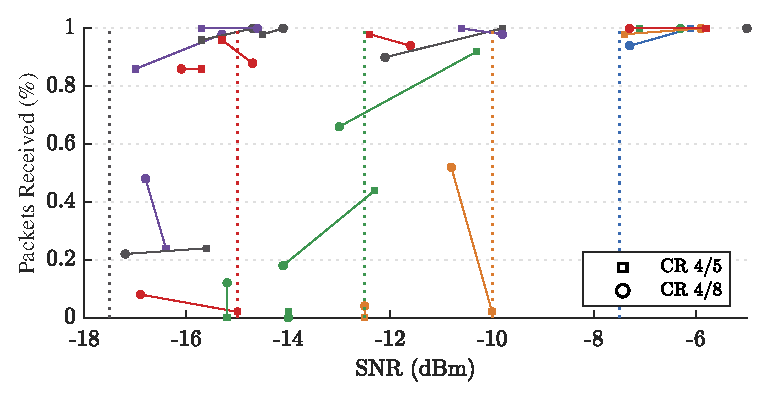
\includegraphics{Figures/cr_pp_plot}
    \caption[Effect of Coding Rate on \ac{snr} and \ac{prp}]{
    Plot of \ac{snr} and \ac{prp} for varying \ac{cr}s. Only configurations where all other factors are identical are included (e.g. height, location, packet length). A line joins each set of points with a matching configuration. \ac{sf} colouring from previous figures is applied to highlight when \ac{snr} limits start to reduce receive probability. When $SNR > -5$, the \ac{prp} is nearly always 100\% and is therefore excluded. Visual indications are that there is little pattern in the data with 4/5s sometimes outperforming 4/8s and vice versa.
    }
    \label{fig:cr_pp_plot}
\end{figure}

\begin{figure}[H]
    \centering
   	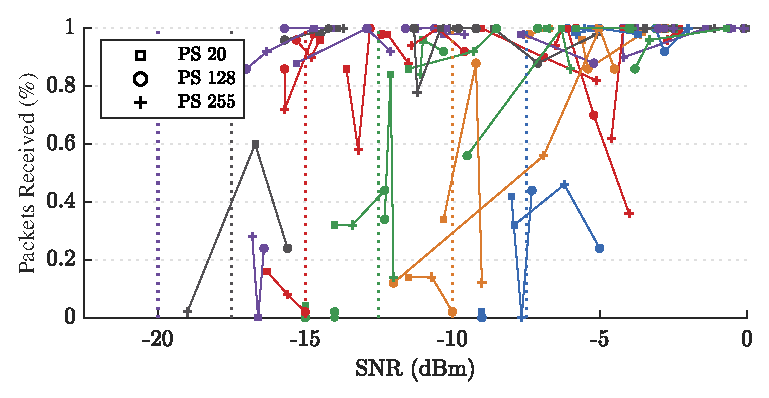
\includegraphics{Figures/pl_pp_plot}
    \caption[Effect of Packet Length on \ac{snr} and \ac{prp}]{
    Plot of \ac{snr} and \ac{prp} for varying packet lengths. Only configurations where all other factors are identical are included. A line joins each set of points with a matching configuration. \ac{sf} colouring from previous figures is applied to highlight when \ac{snr} limits start to reduce receive probability. When $SNR > 0$, the \ac{prp} is nearly always 100\% and is therefore excluded. Visual indications are that the longer packet lengths have a lower \ac{prp}.
    }
    \label{fig:pl_pp_plot}
\end{figure}

\subsection{Environment Effects}
Free-space is the least attenuating environment possible and as such a transmission in free-space should represent the minimum path loss over a given distance; directly leading to the maximum transmission distance. The minimum free space path loss (\ac{fspl}), is calculated as $20\log_{10}(d) + 20\log_{10}(f) - 27.55$ where $d$ is distance in meters and $f$ is frequency in MHz \cite{3YP:ANTENNA_BOOK}. A more reasonable estimate must take into account effects such as ground reflection. The plain earth (\ac{pe}) model considers this and is calculated as $40\log_{10}(d) - 20\log_{10}(h_r) - 20\log_{10}(h_t)$ \cite{3YP:COMBINING_MODELS}. These are all plotted on Figure \ref{fig:distance_pl_plot}. Although transmissions occur at $0.0m$, receiver height ($h_r$) and transmitter height ($h_t$) are measured as the top of the antenna ($h_r = h_t = 0.17m$). As neither model fits the test data, with \ac{fspl} underestimating and \ac{pe} overestimating path loss, an empirical log-model is calculated as $83\log_{10}(d+178)-117$ (E-FSPL). This model fits the curve well but does not necessarily capture the variance caused by fading, as is reflected by only 71\% of data points falling in the 90\% confidence bound. 

\begin{figure}[H]
    \centering
   	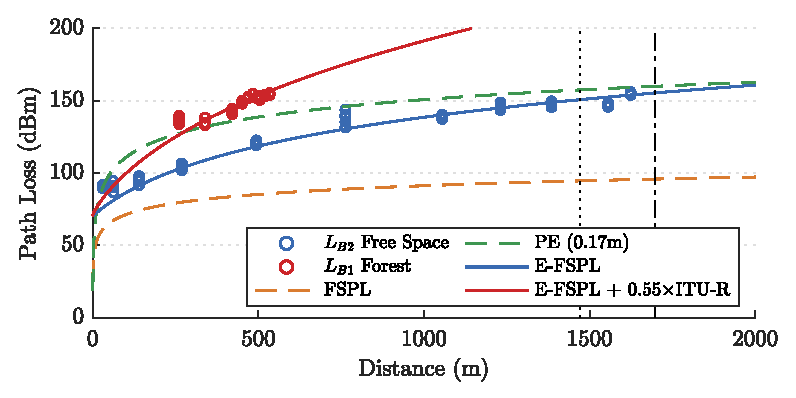
\includegraphics{Figures/distance_pl_plot}
    \caption[Effect of Distance on ground level Path Loss]{
    	Plot of path loss for ground level transmissions through free-space ($L_{B2}$) and forest environments ($L_{B1}$). The \ac{los} horizon and radio horizon are identified as the black dotted and dashed lines respectively.
    }
    \label{fig:distance_pl_plot}
\end{figure}

Forests have high attenuation and should significantly increase path loss and reduce transmission distance. Due to the differences and complexity of vegetation, there is no de-facto propagation model, however, path loss should approximately match that of a vegetation model added to the environment's free space model \cite{3YP:COMBINING_MODELS}.  Many are explained in \cite{3YP:PROP_MODELS}, each of which can be made more flexible by applying an empirical multiplier, giving $L_{Total} = L_{FS} + \beta \times L_{Veg}$ \cite{3YP:EMPIRICAL_MULTIPLIER}. The in-forest model demonstrated is the free-space-fit model with the ITU-R vegetation model, where $\beta=0.55$. The model fits the in-forest test data; giving confidence in both the free-space fit model and that in-forest behaviour follows that of generalised \ac{rf} transmissions. Inter-transmission variance can be attributed to fading, however, it should be noted that test execution was inconsistent when approaching the transmission limit (480m+). This is likely a result of the bearing change between transmitter and receiver causing significant changes to the \ac{los} obstacles. To model this, either individual objects could be modelled or a varying empirical multiplier could be used. Although both the free-space and in-forest fit models serve the purpose of describing the test data, a full assessment of their generalisation would require significantly more test data.

Transmissions at 868MHz are classed as ultra-high-frequency and usually have a maximum distance somewhere between the visual-horizon and radio-horizon \cite{3YP:ANTENNA_BOOK}. They are also susceptible to ground plane effects which can increase path loss. Varying radio heights for comparable measurements are plotted in Figure \ref{fig:height_pl_plot}. The decrease in path loss is clearly seen for both $0.0m\rightarrow 1.0m $ and $0.5m\rightarrow 1.0m$. The effect is less clear for $0.0m\rightarrow 0.5m$. In free-space with $d=10m$ on grass: path-loss for $0.0m$, $0.5m$ and $1.0m$ is 87dBm, 84dBm and 64dBm respectively. The increase between $0.0m$ and $0.5m$ is mathematically significant ($p=0.0$) but of an insignificant degree compared to $0.5m\rightarrow 1.0m$. These results are in-line with the principle that the ground effect is insignificant once antenna height is more than a few wavelengths \cite{3YP:ANTENNA_BOOK}. It is probable that transmissions are limited by the horizon in free-space, as furthest receivable transmissions occur between the horizons for both $0.0m$ and $0.5m$. Most notably there is a sudden increase in path loss between the horizons for $0.0m$.

\begin{figure}[H]
    \centering
   	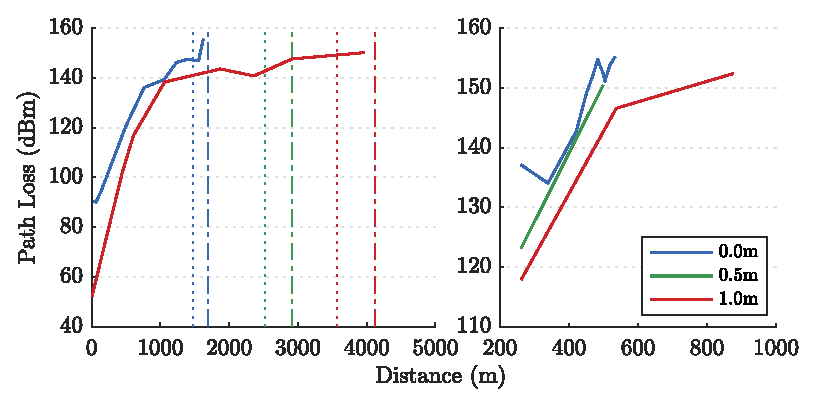
\includegraphics{Figures/height_pl_plot}
    \caption[Effect of Antenna Height on Path Loss]{
		Plot of path loss for varying heights in free-space (left) and in-forest (right). Path loss is the mean of all tests at location. The dotted lines identify the \ac{los} horizons. The dashed lines identify the radio horizons. Directly comparable data was not recorded for free-space 0.5m over multiple distances.
    }
    \label{fig:height_pl_plot}
\end{figure}